%; whizzy chapter$B!!(B-dvi
% -initex iniptex -latex platex -format platex -bibtex jbibtex -fmt fmt
% $B0J>e(B whizzytex $B$r;HMQ$9$k>l9g$N@_Dj!#(B

%     Tokyo Debian Meeting resources
%     Copyright (C) 2012 Junichi Uekawa
%     Copyright (C) 2012 Nobuhiro Iwamatsu

%     This program is free software; you can redistribute it and/or modify
%     it under the terms of the GNU General Public License as published by
%     the Free Software Foundation; either version 2 of the License, or
%     (at your option) any later version.

%     This program is distributed in the hope that it will be useful,
%     but WITHOUT ANY WARRANTY; without even the implied warranty of
%     MERCHANTABILITY or FITNESS FOR A PARTICULAR PURPOSE.  See the
%     GNU General Public License for more details.

%     You should have received a copy of the GNU General Public License
%     along with this program; if not, write to the Free Software
%     Foundation, Inc., 51 Franklin St, Fifth Floor, Boston, MA  02110-1301 USA

%  preview (shell-command (concat "evince " (replace-regexp-in-string "tex$" "pdf"(buffer-file-name)) "&"))
% $B2hA|%U%!%$%k$r=hM}$9$k$?$a$K$O(Bebb$B$rMxMQ$7$F(Bboundingbox$B$r:n@.!#(B
%(shell-command "cd image201205; ebb *.png")

%%$B$3$3$+$i%X%C%@3+;O!#(B

\documentclass[mingoth,a4paper]{jsarticle}
\usepackage{monthlyreport}

% $BF|IU$rDj5A$9$k!"Kh7nJQ$o$j$^$9!#(B
\newcommand{\debmtgyear}{2012}
\newcommand{\debmtgmonth}{11}
\newcommand{\debmtgdate}{17}
% (+ (* (- 2012 2005) 12) 10 -1) started from zero
\newcommand{\debmtgnumber}{94}

\begin{document}

\begin{titlepage}
\thispagestyle{empty}
% $B%?%$%H%k%Z!<%8(B:$BJT=8I,MW$JItJ,$O:G=i$N%^%/%m$KHt$P$9$3$H(B

\vspace*{-2cm}
$BBh(B\debmtgnumber{}$B2s(B $BEl5~%(%j%"(B Debian $BJY6/2q;qNA(B\\
\hspace*{-2cm}

\includegraphics{image2012-natsu/dotdeb.pdf}\\
\hfill{}\debmtgyear{}$BG/(B\debmtgmonth{}$B7n(B\debmtgdate{}$BF|(B

% $B$3$3$O%"%C%W%G!<%H$9$k$3$H(B
% $BA43QJ8;z$K$7$J$$$H%U%)%s%H$N%5%$%:$,9g$o$J$$$N$GCm0U(B
% TODO(uekawa): $B$J$s$G$=$&$J$k$N$+3NG'(B
\rotatebox{10}{\fontsize{32}{32} {\gt $BFC=8(B: $B#L#i#n#u#x!!#p#e#r#f(B}}\\
\rotatebox{10}{\fontsize{32}{32} {\gt $BFC=8(B: $B#B#l#u#e#t#o#o#t#h(B $B#T#e#t#h#e#r(B}}\\

\vspace*{-2cm}
\hfill{}
\includegraphics[height=6cm]{image200502/openlogo-nd.eps}
\end{titlepage}

% Title should be in Japanese text so that we can use it as lint for PDF shiori.
\dancersection{$B$O$8$a$K(B}{$B>e@n(B $B=c0l(B}

\begin{multicols}{2}
 

 $B:#7n$N(BDebian$BJY6/2q$X$h$&$3$=!#$3$l$+$i(BDebian$B$N@$3&$K$"$7$rF'$_F~$l$k$H(B
 $B$$$&J}$b!"$9$G$K$I$C$W$j$H$D$+$C$F$$$k$H$$$&J}$b!"7n$K0l2s(BDebian$B$K$D$$(B
 $B$F8l$j$^$;$s$+!)(B

 Debian$BJY6/2q$NL\E*$O2<5-$G$9!#(B

 \begin{itemize}
 \item \underline{Debian Developer} ($B3+H/<T(B)$B$N0i@.!#(B
 \item $BF|K\8l$G$N!V(B\underline{$B3+H/$K4X$9$k>pJs(B}$B!W$r@0M}$7$F$^$H$a!"%"%C%W%G!<%H$9$k!#(B
 \item \underline{$B>l(B}$B$NDs6!!#(B
 \begin{itemize}
  \item $BIaCJ$P$i$P$i$J>l=j$K$$$k?M!9$,(B face-to-face $B$G=P2q$($k>l$rDs6!(B
	$B$9$k!#(B
  \item Debian $B$N$?$a$K$J$k$3$H$r8l$k>l$rDs6!$9$k!#(B
  \item Debian$B$K$D$$$F8l$k>l$rDs6!$9$k!#(B
 \end{itemize}
 \end{itemize}		

 Debian$B$NJY6/2q$H$$$&$3$H$G5f6KE*$K$O;22C<TA40w$,(BDebian Package$B$r$,$j$,$j(B
 $B$H:n$k%9!<%Q!<%O%C%+!<$K$J$C$?;Q$rLQA[$7$F$$$^$9!#>pJs$N6&M-!&3hMQ$rDL$7(B
 $B$F(B Debian$B$N:#8e$NG=F0E*$JE83+$X$NEZBf$H$7$F!"!V>l!W$H$7$F$N6u4V$rDs6!$9(B
 $B$k$N$,L\E*$G$9!#(B

\end{multicols}

\newpage

\begin{minipage}[b]{0.2\hsize}
 \definecolor{titleback}{gray}{0.9}
 \colorbox{titleback}{\rotatebox{90}{\fontsize{80}{80} {\gt $B%G%S%"%sJY6/2q(B} }}
\end{minipage}
\begin{minipage}[b]{0.8\hsize}
\hrule
\vspace{2mm}
\hrule
\begin{multicols}{2}
\tableofcontents
\end{multicols}
\vspace{2mm}
\hrule
\end{minipage}

\dancersection{$B;vA02]Bj(B}{$B>e@n(B $B=c0l(B}

$B:#2s$N;vA02]Bj$O0J2<$G$9(B:
\begin{enumerate}
 \item Debian $B$G:#$$$^$$$A%5%]!<%H$5$l$F$$$J$$5!G=!"$$$1$F$J$$<BAu$K$D$$$F8l$C$F$/$@$5$$!#(B
\end{enumerate}
$B$3$N2]Bj$KBP$7$FDs=P$$$?$@$$$?FbMF$O0J2<$G$9!#(B
\begin{multicols}{2}
{\small
%; whizzy-master ../debianmeetingresume201211.tex
% $B0J>e$N@_Dj$r$7$F$$$k$?$a!"$3$N%U%!%$%k$G(B M-x whizzytex $B$9$k$H!"(Bwhizzytex$B$,MxMQ$G$-$^$9!#(B
%

\begin{prework}{ koedoyoshida }

\begin{itemize}
 \item Wheezy$B%$%s%9%H!<%i$N%Q!<%F%#%7%g%s9=@.;~$N%G!<%?>C5nBT$A;~4V!#(B
 $B0E9f2=%Q!<%F%#%7%g%s$r:n$m$&$H$9$k$H2L$F$7$J$/BT$?$5$l$k!#(B
 \item 
 Wheezy$B$NJI;f!#$$$1$F$J$$46$8$G(BOSC$B$H$+$NE8<($GE,Ev$J$b$N$rA*$V$N$,LLE]$G7k6I(Bsqueeze$B$d(BDebian$B$N(B($B2a5n$N(B)$B%8%'%M%j%C%/$J$b$N$rA*$V$3$H$K(B...
 \item 
 $B%G%P%C%0%7%s%\%k$r4^$s$@%P%$%J%j$,$J$$!#(B
 $B0JA0BgE}0l$G4d>>$5$s$,H/I=$7$F$$$?OC$,?J$s$G$$$k$H$&$l$7$$!#(B
\end{itemize}

\end{prework}

\begin{prework}{ $B%-%?%O%i(B }

$B;d$,;HMQ$9$kHO0O$G$O$"$j$^$;$s!#(B

\end{prework}

\begin{prework}{ MATOHARA }

$B$"$^$j;W$$$D$+$J$$$G$9$,!"?M$HOC$r$7$F$$$k$H$-0J2<$N$h$&$J$3$H$r8@$o$l$?$3$H$,$"$j$^$9!#(B
\begin{itemize}
 \item 
 Debian$B$O5,DjCM$N@_Dj$,$$$1$F$J$$$N$G@_Dj$rBt;3$$$8$i$J$$$H1?MQ=PMh$J$/$F9)?t$,L5BL$K3]$+$k(B
 \item 
 Debian$B$O%$%s%9%H!<%k$,Fq$7$$(B
\end{itemize}
$B6qBNNc$rJ9$1$J$+$C$?$N$G$9$,!"@_Dj$K$D$$$F$O@i:9K|JL$J$N$G$=$N?M$K$H$C$F(B
 $B8~$$$F$$$J$+$C$?$+$i$H8@$C$F%@%a$+$H$$$&$H$=$&$G$O$J$$$H;W$$$^$9!#(B
$B$7$+$7!"(BopenSUSE $B$N(BYaST $B$O0l85E*$K4IM}$G$-$FJXMx$=$&$@$J$H$O;W$$$^$9!#(B
$B%$%s%9%H!<%k$,Fq$7$$$H$$$&$N$b@N$N%$%a!<%8$J$N$+8=:_$N$3$H$r8@$C$F$$$k$NITL@$J$N$G$9$,!"%G%9%/%H%C%W8~$1$N%G%#%9%H%j%S%e!<%7%g%s$KHf$Y$k$HA*Br;h$,B?$$$N$GFq$7$/46$8$i$l$k$N$+$b$7$l$^$;$s!#(B

\end{prework}

\begin{prework}{ $BNkLZ?rJ8(B }

$B8=:_$O2~A1$7$F$$$k$+$b$7$l$^$;$s$,!"0lIt(Bkernel$B$N%Q%C%1!<%8$K$h$C$F$O(Bdbg$B%Q%C%1!<%8$,L5$$$b$N$,$"$C$?$j$7$F!":$$C$?7P83$,$"$j$^$7$?!#(B
\end{prework}

\begin{prework}{ $BLnEg!!5.1Q(B }

Debian$B$G$$$1$F$$$J$$5!G=!?<BAu$H$$$o$l$k$H!"(B

\begin{itemize}
 \item  ifupdown$B%Q%C%1!<%8(B
 \item  Solaris10$B0J>e$G$$$&$H$3$m$N(BFMD$B$H$+!"(BSVC$BM_$7$$!#(B
 \item  $B%$%s%9%H!<%i$G(B'/'$BA4It(BBTFS$B$H$$$&$NA*Br2DG=$G$7$?$C$1!)(B
 \item  WEB$BMm$_$G!":G?7(BWEB$B3+H/4X780l<0$N%Q%C%1!<%8%j%]%8%H%j$H$$$&$N$,M_$7$$5$$,$9$k!J(BWEB$B%7%9%F%`$GN.9T$j$b$N$d$i!"NI$/;H$o$l$F$$$=$&$J%P!<%8%g%s$N%=%U%H$KFC2=$7$?%j%]%8%H%j!#$=$l$J$i(Bexperimental$B$7$+B8:_$7$J$$$H$+$G$b%$%$!*!K(B
 \item  Debian$B$H$O$A$g$C$H%:%l$F$k$+$b$7$l$^$;$s$,!"(Bsynaptic$B$O(B...iTunes$B$_$?$$$K$J$C$F$[$7!<(B
\end{itemize}

$B$H8@$$$?$$J|Bj8@$C$F$_$?!#(B
\end{prework}

\begin{prework}{ $B>e@n=c0l(B }

Android $BMQ$N(BADB$B%3%^%s%I$H$+$,I8=`$GF~$C$F$$$k$H4r$7$$$J$!!#(B
\end{prework}

\begin{prework}{ yamamoto }

Debian $B$NM}A[$H?.G0$OBg9%$-$J$s$G$9$,!">/$75$$K$J$kE@$b$"$j$^$9!#(B

$BNc$($P(B Debian-Installer $B$K$O(B non-free $B$GHRI[$5$l$F$$$k(B firmware $B%Q%C%1!<%8$,4^$^$l$F$$$J$$E@$J$I$G$9!#(Bnon-free $B$N%Q%C%1!<%8$O!"MM!9$JM}M3$G(B non-free $B$KJ,N`$5$l$F$$$k$o$1$G$9$,!"$=$N0l$D$K%F%-%9%H$N%=!<%9$,B8:_$7$J$$$?$a!"$H$+$$$&M}M3$b$"$j$^$9!#(B

$BJL$K!V(Bnon-free $B$K$9$k$J!W$H$+<gD%$7$?$$$o$1$G$O$J$$$N$G$9$,!"HRI[$N@)8B$NL5$$%Q%C%1!<%8$^$G!V(Bnon-free $B$@$+$i!W$H!"<}O?$r5q@d$9$k$N$O>/!9$d$j$9$.$G$O$J$$$+$H9M$($F$$$^$9!#(B
\end{prework}

\begin{prework}{ $BLn<s(B }

\begin{itemize}
 \item $B%Q%C%1!<%8$N%j%9%H%"$K(Bdpkg --get-selections$B$O$A$g$C$HHyL/(B
 \item aptitude-run-state-bundle$B$O$$$^$$$AMQES$,$o$+$i$J$$(B
 \item stable$B$K$?$^$K;H$$J*$K$J$i$J$$%Q%C%1!<%8$,$"$k(B
       \begin{itemize}
	\item $B8E$9$.$k$+$i$H$+(B($BNc(B: lxc)
       \end{itemize}

 \item $B%Q%C%1!<%8$N%H%i%s%6%/%7%g%s$,M_$7$$(B
       \begin{itemize}
	\item $B0lEY%$%s%9%H!<%k$7$F$_$F$*$+$7$+$C$?$i(Brevert
	\item $BLdBj$J$1$l$P(Bcommit$B$_$?$$$J(B
       \end{itemize} 
\item multiarch$B$OF3F~$7$FK\Ev$KNI$+$C$?$N$+(B?
\end{itemize}

\end{prework}

\begin{prework}{ $BF|HfLn(B $B7<(B }

$B;H$$$3$_$,B-$j$F$J$$$N$+$b$7$l$^$;$s$,!"(B
$BMzNr4IM}%7%9%F%`$KJ]B8$5$l$F$$$k(Btree$B$r(B
debian$B%Q%C%1!<%8$H$7$F(B build $B$7$?$j(B
install $B$7$?$j$9$k$H$-$KJXMx$J%D!<%k$,(B
$B$"$^$jL5$$$N$+$b$H;W$$$^$7$?!#(B

\end{prework}

\begin{prework}{ dictoss($B?yK\!!E5=<(B) }

iptables$B$N%3%^%s%I0z?t$,B>$N(BOS$B$H0c$&$h$&$J46$8$,$9$k!#$=$N$?$a(Biptables$B$N=i?4<T$,(Bweb$B$GD4$Y$?%3%^%s%I$r<B9T$7$F$b9=J8%(%i!<$G$O$8$+$l$F?I$$!#(B
\end{prework}

}
\end{multicols}

\dancersection{Debian Trivia Quiz}{$B>e@n=c0l(B}

$B$H$3$m$G!"$_$J$5$s(B Debian $B4XO"$NOCBj$K$*$$$D$$$F$$$^$9$+!)(BDebian$B4XO"$NOC(B
$BBj$O%a!<%j%s%0%j%9%H$r$h$s$G$$$k$HDI@W$G$-$^$9!#$?$@$h$s$G$$$k$@$1$G$O$O(B
$B$j$"$$$,$J$$$N$G!"M}2rEY$N%F%9%H$r$7$^$9!#FC$K0l?M$@$1$G$O0UL#$,$o$+$i$J(B
$B$$$H$3$m$b$"$k$+$bCN$l$^$;$s!#$_$s$J$G0l=o$KFI$s$G$_$^$7$g$&!#(B

$B:#2s$N=PBjHO0O$O(B\url{debian-devel-announce@lists.deban.org} $B$d(B \url{debian-d\
evel@lists.deban.org}$B$KEj9F$5$l$?(B
$BFbMF$H(BDebian Project News$B$+$i$G$9!#(B

\begin{multicols}{2}
%; whizzy-master ../debianmeetingresume201211.tex
% $B0J>e$N@_Dj$r$7$F$$$k$?$a!"$3$N%U%!%$%k$G(B M-x whizzytex $B$9$k$H!"(Bwhizzytex$B$,MxMQ$G$-$^$9!#(B
%

\santaku
{FTP master $B$K$"$?$i$7$/;22C$7$?$N$O(B}
{iwamatsu}
{ansgar}
{bdale}
{B}
{Ansgar $B$,?7$7$/;22C$7$^$7$?!#(Bmhy, joerg, ansgar $B$N;0?MBN@)$K(B}

\santaku
{pdiff$B$G2?$,2~A1$5$l$?$+(B}
{$B:GBg(B2$B$D$N(BDiff$B$r%@%&%s%m!<%I$9$l$PNI$$$h$&$KJQ99$K$J$C$?(B}
{$B0lF|(B10$B8D$E$D(BDiff$B$r@8@.$9$k$h$&$K$J$C$?(B}
{Diff$B$C$F$J$K$=$l$*$$$7$$$N!)(B}
{A}
{apt-get update $B$NCY$5$,%^%7$K$J$j$^$9$M!#(B}

\santaku
{CTTE 573745 $B$G2?$,7hDj$5$l$?$+(B}
{Mattias Klose $B%/%S(B}
{python $B=*N;$N$*CN$i$;(B}
{$B$_$s$JCgNI$/$7$h$&$M(B}
{C}
{python $B$N%a%s%F%J$N%3%_%e%K%1!<%7%g%sITB-$K$D$$$F$N5DO@$O7k6I$_$s$JCgNI(B
$B$/$7$^$7$g$&$H$$$&7kO@$K$J$j$^$7$?$M!#(B}

\santaku
{$B?7$7$/(BFront Desk$B$N%a%s%P!<$K$J$C$?$N$O(B}
{Kouhei Maeda}
{Iwamatsu}
{Jonathan Wiltshire}
{C}
{4$B?M$K$J$j$^$7$?!'(B
 Bernd Zeimetz      (bzed)
 Enrico Zini        (enrico)
 Jan Hauke Rahm     (jhr)
 Jonathan Wiltshire (jmw)
}

\santaku
{debian installer 7.0 beta3 $B$N?75!G=$G$O$J$$$N$O$I$l$+(B}
{ipv6}
{UEFI}
{grub2}
{C}
{}

\santaku
{}
{}
{}
{}
{}
{}
\santaku
{}
{}
{}
{}
{}
{}
\santaku
{}
{}
{}
{}
{}
{}
\santaku
{}
{}
{}
{}
{}
{}

\end{multicols}

%-------------------------------------------------------------------------------
\dancersection{Android $B7HBS$G(BBluetooth Tethering}{$B>e@n=c0l(B}
%-------------------------------------------------------------------------------
\index{bluetooth}
\index{bluetooth tethering}
\index{tethering}

\subsection{$B$O$8$a$K(B}

$B:G6a$N(BAndroid$B7HBS$b%Q%=%3%s$b(BBluetooth$B$KBP1~$7$F$$$^$9!#$=$7$F(BBluetooth
profile$B$G$"$k(BPAN$B$d(BDUN$B$KBP1~$7$F$$$k$b$N$bB?$$$h$&$G$9!#(B
Android 4.0$B$"$?$j$GBP1~$9$k$h$&$K$J$C$?$H;W$o$l$k(BBluetooth Tethering$B$rMx(B
$BMQ$9$k$3$H$G(BAndroid$B7HBS$K(BBluetooth PAN $B7PM3$G@\B3$7!"(BAndroid$B7HBS$N2s@~$r(B
$BMxMQ$7$F30It$N%M%C%H%o!<%/$K@\B3$G$-$k$h$&$K$J$j$^$9!#(B

WiFi Tethering$B$N$h$&$KEENO>CHq$,9b$9$.$k$N$GKh2s@_Dj$G%*%U$K$9$kI,MW$,$"(B
$B$k$k$H$$$&$3$H$b$J$/!"$d(BUSB Tethering$B$N$h$&$KKh2sJ*M}E*$K@\B3$9$kI,MW$b$J(B
$B$$$N$GJXMx$G$9!#(B
$B%+%P%s$NCf$K7HBS$r$$$l$?$^$^@\B3$G$-$k$N$G5$3Z$G$9$h!#(B

\subsection{$B@_DjJ}K!(B}

Android$B7HBSB&$G$O(BBluetooth Tethering$B$r%*%s$K$7$^$9!#(B

$B$"$H!"(BBluetooth$B$N%Z%"%j%s%0$r9T$$$^$9!#7HBSEEOCB&$N@_Dj$G2D;k>uBV$K$7$F(B
$B$*$$$F(BGNOME$B$N@_Dj$GDI2C$9$l$P$h$$$G$7$g$&!#(B(\fgref{fig:gnome-bt2})

\begin{figure}[ht]
 \begin{center}
  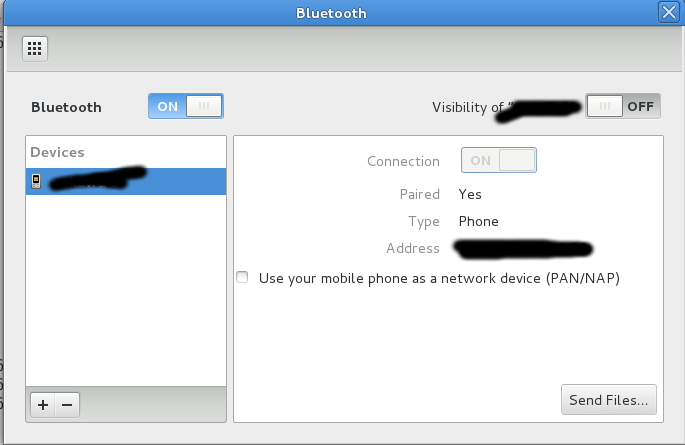
\includegraphics[width=0.5\hsize]{image201211/bt2.png}
  \label{fig:gnome-bt2}
 \end{center}
\end{figure}

$B0lC6@_Dj$7$F$*$/$H%M%C%H%o!<%/$NA*Br8uJd$K(BMobile Broadband$B$H$$$&$N$,8=$l(B
$B$F$=$3$G7HBSEEOC$N(BBluetooth PAN$B@\B3$,A*Br$G$-$k$h$&$K$J$j$^$9!#(B

\begin{figure}[ht]
 \begin{center}
  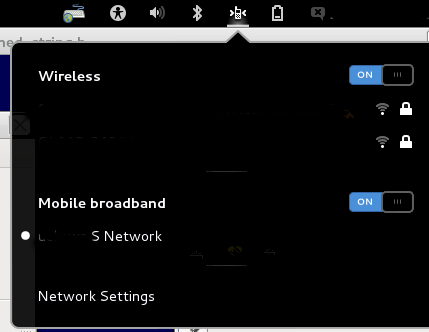
\includegraphics[width=0.5\hsize]{image201211/bt1.png}
  \label{fig:gnome-bt1}
 \end{center}
\end{figure}

\subsection{$B%M%C%H%o!<%/9=@.(B}

Linux $BB&$+$i$O(Bbnep0 $B%G%P%$%9$H$7$F8+$($^$9!#J#?t%^%7%s$+$i@\B3$9$k$H$=$l(B
$B$>$l$,JL$N%5%V%M%C%H$K@\B3$5$l$k$C$]$$$N$G$*8_$$$KDL?.$O$G$-$J$$$h$&$G$9!#(B
WiFi Tethering$B$@$HF1$8%5%V%M%C%H$K$D$J$,$k$N$G8D?ME*$K$O%&%'%V%5!<%P!<$H(B
$B%/%i%$%"%s%H$r@\B3$9$k$?$a$N%O%V$H$7$FJXMx$KMxMQ$7$F$$$?$N$G$9$,!"$=$&$$(B
$B$&;H$$J}$O$G$-$J$$$h$&$G$9!#(B

\begin{commandline}
bnep0     Link encap:Ethernet  HWaddr 
          inet addr:192.168.46.43  Bcast:192.168.46.255  Mask:255.255.255.0
\end{commandline}

\subsection{$B$^$H$a(B}

Bluetooth PAN$B$OJXMx!"$H$$$&$3$H$G$7$?!#$?$@!"$J$<$@$+F|K\$N7HBSEEOC$O(B
Bluetooth PAN$B$KBP1~$7$F$J$$$b$N$,B?$/!"$^$?3$307HBS$NF|K\%b%G%k$O$=$N5!G=(B
$B$r:o$C$F$?$j$9$k$b$N$,$"$j$^$9(B\footnote{$BNc!'I.<T$N=jM-$9$k(BGalaxy Nexus
DoCoMo$BHG(B}$B!#$3$3$O$<$R(BBluetooth PAN$BBP1~$8$c$J$$7HBSEEOC$O9XF~$7$J$$$3$H$G(B
$B>CHq<T$N0U8+$rI=L@$7$F$/$@$5$$!#(B

%-------------------------------------------------------------------------------
\dancersection{perf $B$G%Q%U%)!<%^%s%9%A%e!<%K%s%0(B}{$B>e@n=c0l(B}
%-------------------------------------------------------------------------------
\index{perf}

\subsection{$B$O$8$a$K(B}

$B:G6a$N$?$$$F$$$N(BCPU$B$K$O(BPerformance Counters $B$H$$$&;EAH$_$,$"$j!"FCDj$N%$(B
$B%Y%s%H$,0lDj2s?tH/@8$7$?$i$"$k=hM}$r$9$k$H$$$&;v$,$G$-$k$h$&$K$J$C$F$$$^(B
$B$9!#$=$l$rMxMQ$7$F%W%m%U%!%$%i!<$,<BAu$G$-$F!"%W%m%0%i%`$N%Q%U%)!<%^%s%9(B
$B%\%H%k%M%C%/$NH/8+$KLrN)$F$k$3$H$,$G$-$^$9!#(B
$B@N$O(B oprofile $B$r;H$C$F$$$?$N$G$9$,!":G6a$N(BLinux $B%+!<%M%k$G$O(B perf $B$H$$$&(B
$B;EAH$_$r;H$&$N$,<gN.$N$h$&$G$9!#(B

$B%+!<%M%kB&$N%5%]!<%H$OI8=`$GF~$C$F$$$^$9!#%3%^%s%I%i%$%s$N(B perf $B%3%^%s%I(B
$B$O(B linux-base $B%Q%C%1!<%8$K$O$$$C$F$$$F$?$$$F$$$N4D6-$G$OI8=`$G%$%s%9%H!<(B
$B%k$5$l$F$$$k$h$&$K$_$($k$N$G$9$,<BBN$O%+!<%M%k$K$"$C$?%P!<%8%g%s$rDI2C$G(B
$B%$%s%9%H!<%k$9$kI,MW$,$"$j$^$9!#Nc$($P!"(Blinux 3.2 $B$@$H(B linux-tools-3.2 $B$r(B
$B%$%s%9%H!<%k$9$k$3$H$K$J$j$^$9!#(B

\begin{commandline}
 $ uname -r
3.2.0-3-amd64
 $ sudo apt-get install linux-tools-3.2
\end{commandline}
\index{linux-tools-3.2}

$B%G%P%C%0%7%s%\%k$,$"$k$H4X?tL>$H$+$,$-$l$$$K=P$k5$$,$9$k$N$GMxMQ$7$F$$$k(B
$B%i%$%V%i%j$N%G%P%C%0%7%s%\%k$b$$$l$F$*$/$H$h$$$G$7$g$&!#I8=`%i%$%V%i%j$O(B
$B$$$l$F$*$-$^$7$g$&!#(B

\begin{commandline}
 $ sudo apt-get install libc6-dbg libstdc++6-4.7-dbg
\end{commandline}
%$

\subsection{perf stat}

$B%W%m%0%i%`C1BN$N<B9T;~4V$r7WB,$7$F%l%]!<%H$7$F$/$l$k%3%^%s%I$H$7$F(B time$B%3(B
$B%^%s%I$,$"$j$^$9$,!"$=$NBe$o$j$K$D$+$($=$&$J%D!<%k$H$7$F!"(B perf stat $B$,$"(B
$B$j$^$9!#:G6a$N(BCPU$B$OIi2Y$K$h$C$F(BCPU$B<~GH?t$,JQ$o$j!"$=$&$$$&%7%9%F%`$K$*$$(B
$B$F%Q%U%)!<%^%s%9$NB,Dj$N$?$a$K<B9T;~4V$@$1$r7WB,$9$k$H$$$&$N$OE,@Z$G$O$J(B
$B$$$N$G$9$,!"(Bperf stat$B$O$=$l0J30$KI,MW$=$&$JCM$r7WB,$7$F$/$l$k$N$GJXMx$G$9!#(B

\begin{commandline}
$ perf stat ./apt-index-cmd debian_dists_sid_main_binary-amd64_Packages debian > /dev/null
 Performance counter stats for './apt-index-cmd debian_dists_sid_main_binary-amd64_Packages debian':

       1741.828818 task-clock                #    0.997 CPUs utilized          
               165 context-switches          #    0.000 M/sec                  
                 6 CPU-migrations            #    0.000 M/sec                  
            27,392 page-faults               #    0.016 M/sec                  
     4,990,934,326 cycles                    #    2.865 GHz                     [83.29%]
     1,681,297,382 stalled-cycles-frontend   #   33.69% frontend cycles idle    [83.27%]
     1,096,373,883 stalled-cycles-backend    #   21.97% backend  cycles idle    [66.62%]
     7,738,965,303 instructions              #    1.55  insns per cycle        
                                             #    0.22  stalled cycles per insn [83.51%]
     1,784,494,907 branches                  # 1024.495 M/sec                   [83.49%]
        32,701,183 branch-misses             #    1.83% of all branches         [83.32%]

       1.746581711 seconds time elapsed
\end{commandline}
  
\subsection{perf record}

perf record $B%3%^%s%I$O%W%m%U%!%$%k>pJs$r5-O?$9$kL?Na$G$9!#%Q%i%a!<%?$H$7(B
$B$F;XDj$7$?%3%^%s%I$r$=$N$^$^<B9T$7$F!"%+%l%s%H%G%#%l%/%H%j$K(B perf.data$B%U%!(B
$B%$%k$r:n@.$7$^$9!#8e$K(B perf report $B$J$I$G$=$N%W%m%U%!%$%k%G!<%?$r3NG'$9$k(B
$B$3$H$,$G$-$^$9!#(B

\begin{commandline}
$ perf record ./apt-index-cmd debian_dists_sid_main_binary-amd64_Packages  debian > /dev/null
[ perf record: Woken up 1 times to write data ]
[ perf record: Captured and wrote 0.087 MB perf.data (~3800 samples) ]
$ ls -l perf.data
-rw------- 1 dancer dancer 93560 10$B7n(B 10 07:03 perf.data

\end{commandline}

perf record -g $B%*%W%7%g%s$r$D$1$k$H%3!<%k%0%i%U>pJs$b5-O?$9$k$h$&$G$9!#(B

$B%G%U%)%k%H$O0lIC(B1000$B%5%s%W%k$H$k$h$&$J$N$G!"%W%m%0%i%`$N<B9T;~4V$K1~$8$F(B
$B%5%s%W%k?t$rE,Ev$KD4@0$7$^$7$g$&!#(B $BNc$($PA4BN$G<B9T$,0lIC$G=*$o$C$F$7$^$&(B
$B%W%m%0%i%`$N>l9g$O(B-F 10000 $B$r$D$1$F$_$k$H$h$j%5%s%W%k?t$,$H$l$F$$$$$+$b$7(B
$B$l$^$;$s!#(B

\subsubsection{gcc $B$N%3%s%Q%$%k%*%W%7%g%s$N8!F$(B}

gcc $B$G%=!<%9%3!<%I%3%s%Q%$%k$9$k$H$-$K!"(B-g $B%*%W%7%g%s$r$D$1$k$H%G%P%C%0>p(B
$BJs$,$D$-$^$9!#4X?t%7%s%\%k$N>pJs$H$+9T?t$H$+%=!<%9%3!<%I$H$+$,F@$i$l$k$N(B
$B$G$3$l$OB?J,=EMW!#(B

$B%3!<%k%0%i%U$,$"$^$j$J$$$J$!$H;W$C$?$i:GE,2=$N$7$9$.$H%9%?%C%/%H%l!<%9$N(B
$B$H$j$K$/$5$r5?$C$F$_$^$7$g$&!#(B

$BDL>o:GE,2=%*%W%7%g%s(B -O2 $B$r$D$1$F%3%s%Q%$%k$7$^$9$,!"(Bamd64 $B$N>l9g!"(Bgcc $B$G(B
-O2 $B$r$D$1$F%3%s%Q%$%k$9$k$H%U%l!<%`%]%$%s%?$,$J$/$J$C$F%9%?%C%/%H%l!<%9(B
$B$r<hF@$7$K$/$/$J$C$F$$$^$9!#(Blibunwind$B;H$($P<hF@$G$-$k$O$:$G$9$,!"B?J,(B
perf$B$O%+!<%M%k6u4V$G%9%?%C%/%H%l!<%9$r$H$C$F$$$k$N$G$=$&$J$C$F$J$$$C$]$$(B
$B$G$9!#BP:v$H$7$F<c43%*!<%P!<%X%C%I$,$"$j$^$9$,!"(B-fno-omit-frame-pointer
$B$r;XDj$9$k$H!"%U%l!<%`%]%$%s%?$rA`:n$9$k%3!<%I$r@8@.$7$F$/$l$^$9(B

C++$B$G%U%!%s%/%7%g%s%*%V%8%'%/%H$H$+%F%s%W%l!<%H%W%m%0%i%_%s%0$7$^$/$C$F$$(B
$B$k$H!"4X?t$,$[$H$s$I%$%s%i%$%sE83+$5$l$F$7$^$$!"%3!<%k%0%i%U$K8=$l$kItJ,(B
$B$,>/$J$/$J$j$^$9!#M}2rITG=$K$J$C$F$-$?$i$?$^$K(B -O $B$"$?$j$G%3%s%Q%$%k$7$F(B
$B%9%?%C%/%H%l!<%9$r8+$F$_$^$7$g$&!#(B

\subsection{perf report}

perf report $B%3%^%s%I$O<hF@$7$?%W%m%U%!%$%k%G!<%?$r2D;k2=$9$k%3%^%s%I$G$9!#(B
$B%F%-%9%H%3%s%=!<%k%a%K%e!<7A<0$K$J$C$F$$$F!"5$$K$J$k%7%s%\%k$rA*Br$7$F%=!<(B
$B%9%3!<%I$N%"%N%F!<%7%g%s$r8+$k$3$H$,$G$-$^$9!#$I$N%=!<%9%3!<%I$N9T$KBP1~(B
$B$9$k%"%;%s%V%i$N$I$NL?Na$G(BCPU$B=hM};~4V$rHq$d$7$?$N$+$rI=<($7$F$/$l$^$9!#(B

\begin{commandline}
$ perf report
Events: 1K cycles                                                              
 18.65%  apt-index-cmd  apt-index-cmd        [.] available_parser::AptIndexSpiri
  7.38%  apt-index-cmd  libc-2.13.so         [.] _int_malloc
  6.64%  apt-index-cmd  libc-2.13.so         [.] malloc
  5.17%  apt-index-cmd  libstdc++.so.6.0.17  [.] std::string::_M_replace_aux(uns
  4.03%  apt-index-cmd  libc-2.13.so         [.] _int_free
  4.02%  apt-index-cmd  libstdc++.so.6.0.17  [.] __cxxabiv1::__vmi_class_type_in
  3.81%  apt-index-cmd  libstdc++.so.6.0.17  [.] std::string::_M_mutate(unsigned
  3.59%  apt-index-cmd  libstdc++.so.6.0.17  [.] std::ctype<char> const& std::us
  3.00%  apt-index-cmd  libc-2.13.so         [.] __strcmp_sse42
  2.74%  apt-index-cmd  apt-index-cmd        [.] boost::detail::function::functi
  2.72%  apt-index-cmd  libstdc++.so.6.0.17  [.] __dynamic_cast
  2.67%  apt-index-cmd  libc-2.13.so         [.] free
  2.46%  apt-index-cmd  libc-2.13.so         [.] __memcmp_sse4_1
\end{commandline}

$B$3$3$G%(%s%?!<$r$*$9$H<!$,I=<($5$l(B

\begin{commandline}

available_parser::AptIndexSpirited::MakeIndex()::{lambda(std::vector<char, std::
    0.00 :          40368a:       je     4036ac <available_parser::AptIndexSpir
         :                                                                     
         :          const std::string& get() const { return my_string_; }      
         :                                                                     
         :          // for 'map' comparison.                                   
         :          bool operator<(const OrderedHashedString& b) const {       
         :            if (ordered_hash_ == b.ordered_hash_) {                  
    2.87 :          40368c:       mov    0x28(%rbx),%rdx                       
         :              return my_string_ < b.my_string_;                      
         :            } else {                                                 
         :              return ordered_hash_ < b.ordered_hash_;                
   34.96 :          403690:       cmp    %rbp,%rdx                             
    1.43 :          403693:       setb   %cl                                   
         :                                                                     
         :          const std::string& get() const { return my_string_; }      
         :                                                                     
         :          // for 'map' comparison.                                   
         :          bool operator<(const OrderedHashedString& b) const {       
         :            if (ordered_hash_ == b.ordered_hash_) {                  
  
 \end{commandline}

\subsubsection{C++ $B$N%3!<%I$N>l9g(B}

C++$B$G%F%s%W%l!<%H$r3hMQ$7$F$$$k%3!<%I$rD/$a$k>l9g!"(Bperf report $B$N(BTUI$B%$%s(B
$B%?%U%'!<%9$@$H4X?tL>$,==J,I=<($5$l$J$$$J$HG:$`$3$H$K$J$j$^$9!#$H$j$"$($:(B
TUI$B$8$c$J$$%$%s%?%U%'!<%9$K$9$k$H$b$C$HI=<($5$l$^$9$,!"$$$^$$$AA4BN$OI=<((B
$B$G$-$^$;$s!#(B

$B$?$H$($P4X?tL>$,$3$N$h$&$KESCf$G@Z$l$F$7$^$$$^$9!#$^$@KM$O2sHrJ}K!$rH/8+$7$F(B
$B$$$^$;$s!#(B

\begin{commandline}
 void
 MeasureRaw<std::unordered_map<boost::iterator_range<__gnu_cxx::__normal_iterator<char
 const*, std::string> >, int,
 RangeHash<boost::iterator_range<__gnu_cxx::__normal_iterator<char
 const*, std::string> > >,
 RangeEqualTo<boost::iterator_range<__gnu_cxx::__normal_iterator<char
 const*, std::string> > >,
 std::allocator<std::pair<boost::iterator_range<__gnu_cxx::__normal_iterator<char
 const*, std::string> > const, int> > >, __gnu_cxx::__normal_iterator
\end{commandline}


\dancersection{systemd}{$B4d>>(B $B?.MN(B}
\index{systemd}

\subsection{$B$O$8$a$K(B}
$B@$$NCf$N<gMW$J(BLinux$B%G%#%9%H%j%S%e!<%7%g%s$O(B SysVinit $B$N(B init scripts $B$+$i(B
$BB>$N(Binit $B%7%9%F%`$K0\9T$7$D$D$"$j$^$9!#(B
Fedora$B$d(BArch Linux$B$,(Bsystemd $B$K0\9T$r;O$a$?$H$$$&$3$H$b$"$j!"0lIt$G@9$j>e$,$C$F$$$k(B
$B!J0$I!6+4-$H$b$$$&!K$h$&$G$9!#(B
$B$^$5$+(B $B$$$^$@$K(B SysVinit $B$r;H$C$F$$$k(B Debian$BJY6/2q;22C<T$,$$$k$H$O;W$($^$;$s$,!"(B
$B@9$j>e$,$C$F$$$k$h$&$J$N$G(BDebian$B$H(BSystemd$B$K$D$$$F$^$H$a$F$_$^$7$?!#(B

\subsection{systemd$B$H$O!)(B}

RedHat $B$K6P$a$F$$$k(B Lennart Poettering $B;a$K$h$C$F3+H/$5$l$F$$$k(B init $B$NBeBX%W%m%0%i%`$G$9!#(B
$B<B:]$K$O(B init $B$NBeBX$@$1$G$O$J$/!"(BLinux $B$N%5!<%S%9!J%G!<%b%s!K4IM}%U%l!<%`%o!<%/$H$J$C(B
$B$F$$$^$9!#(B
%Linux $B%+!<%M%kMQ$N%G%P%$%94IM}%D!<%k$G$"$k(B udev $B$,(B systemd $B$N%=!<%9$K%^!<%8(B
%$B$5$l$F$$$^$9!#%m%0%7%9%F%`$b$"$k!#>-Mh$O(B cron $B$d(B acpid $B$J$I$NBeBX$(5!G=$r(B
%$BDs6!$9$kM=Dj$i$7$$!#(B
$B:#$^$G$N(Binit$B%7%9%F%`$N0c$$$O%5!<%S%9$N%W%m%;%94IM}$r(B pid $B$G$O$J$/!"(Bcgroups $B$r;H$&E@$H(B
$B%5!<%S%9$N5/F0$r%=%1%C%H$H%P%9$r;H$&E@$,$"$j$^$9!#$3$l$i$O(B D-Bus $B$r;H$C$F9T$$$^$9!#$3$l$K$h$C$F%7%9%F%`N)$A>e$2=hM}$r$h$jJBNsE*$K9T$($k$h$&$K$J$C$F$$$^$9!#(B
$B$^$?!"(BSystem V $B%9%?%$%k$H(BBSD$B%9%?%$%k$NN>J}$r%5%]!<%H$7$F$$$^$9!#(B

$B3+H/$O(B freedesktop.org
\url{http://cgit.freedesktop.org/systemd/systemd/}
$B$G9T$o$l$F$*$j!"3+H/$O3hH/$G=5$K0lEY$O%P!<%8%g%s%"%C%W$7$F$$$^$9!#(B
$B:G?7%P!<%8%g%s$O(B v195$B$H$J$C$F$$$^$9!#(B

\subsubsection{systemd $B$NMxE@(B}
systemd $B$O(B SysVinit $B$HHf$Y$F<!$N$h$&$JMxE@$,$"$j$^$9!#(B

\begin{itemize}
\item $B@_Dj$,MF0W!#(B\\
SysVinit $B$O%7%'%k%9%/%j%W%H$G5-=R$7$F$$$?$?$a!"3+H/<T$K$h$C$F=q$-J}$,0[$J$j$^$9!#(B
$B$h$C$F@_Dj$dFbMF$NM}2r$,Fq$7$$$3$H$,$"$j$^$9!#(Bsystemd $B$O@_DjJ}K!$d9`L\Ey$,7h$^$C$F$$$k$?$a!"(B
$B@_Dj$7$d$9$/$J$C$F$$$^$9!#(B

\item $B5/F0$,Aa$$!#(B \\
$B%7%'%k$K0MB8$7$F$$$J$$$N$H%G!<%b%s$,JBNs5/F0$9$k$?$a5/F0$,Aa$$$G$9!#(B

\item $B%+!<%M%k%b%8%e!<%k$NA`:n!"%;%C%7%g%s4IM}!"%m%04IM}!"%G%#%9%/$N0E9f2=$J$I$r(B
$BE}9g!#(B

\end{itemize}

$B$=$NB>!":n<T$K$h$k@bL@$r(B\url{http://0pointer.de/blog/projects/why.html}$B$+$i;2>H$G$-$^$9!#(B

\subsection{Debian$B$G;H$&(B}

systemd $B$O$b$A$m$s(B Debian $B$G$bDs6!$5$l$F$*$j!"(Btesting / unsable $B$G(B v44 $B$,(B
$BMxMQ$G$-$^$9!#:G?7HG$H%P!<%8%g%s$K:9$,$"$j$^$9$,!"%"%C%W%9%H%j!<%`$G(B
$BIQHK$K%P!<%8%g%s%"%C%W$9$k$N$G%P!<%8%g%s$O$"$^$jLdBj$G$O$"$j$^$;$s!#(B
v44 $B$G$b(B systemd $B$r==J,$K;H$&$3$H$,$G$-$^$9!#(B

$B$$$^$N$H$3$m(B Debian$B$K4X$9$k>pJs$O(B \url{http://wiki.debian.org/systemd}
$B$K$^$H$^$C$F$$$^$9$,>pJs$,>/$J$/!"FbMF$b8E$$$G$9!#(B

\subsubsection{$B%$%s%9%H!<%k(B}
$B@h$K$b=q$$$?$h$&$K(B Debian$B$G$O(B v44 $B$,:G?7HG$G$9!#(B
apt-get / aptitude $B$G%$%s%9%H!<%k$G$-$^$9!#(B

$B$^$?!"(BLinux $B%+!<%M%k$O(B 2.6.39 $B0J>e!"(Bdevtmpfs, fanotify, autofs4, cgroups $B$,M-8z$K$J$C$F$$$k(B
$BI,MW$,$"$j$^$9!#(B

%\begin{commandline}
%$ uname -a 
%Linux debian 3.2.0-4-amd64 #1 SMP Debian 3.2.32-1 x86_64 GNU/Linux
%\end{commandline}
%$

$B%$%s%9%H!<%k$O0J2<$N$h$&$K<B9T$7$^$9!#(B

\begin{commandline}
$ sudo apt-get install systemd
\end{commandline}
%$

$B0J2<$N%Q%C%1!<%8$,0MB84X78$G%$%s%9%H!<%k$5$l$^$9!#(B
\begin{commandline}
libsystemd-daemon0
libsystemd-id128-0
libsystemd-journal0
libpam-systemd
\end{commandline}
%$

$B<!$K(B $B%V!<%H%m!<%@$K(Binit$B;XDjDI2C$7$^$9!#(Bgrub $B$r;H$C$F$$$k>l9g!"(B\texttt{/etc/default/grub} $B$N(B
\texttt{GRUB\_CMDLINE\_LINUX\_DEFAULT} $B$K(B {\bf init=/lib/systemd/systemd} $B$rDI5-$7$^$9!#(B 

\begin{commandline}
$BJQ99A0(B:
GRUB_CMDLINE_LINUX_DEFAULT="quiet"
$BJQ998e(B:
GRUB_CMDLINE_LINUX_DEFAULT="quiet init=/lib/systemd/systemd"
\end{commandline} 
%$
$BJQ998e!"(B{\bf update-grub}$B$r<B9T$7!"(Bgrub $B$K@_Dj$rH?1G$7$^$9!#(B
$B$=$7$F%j%V!<%H$7$^$9!#(B
$B@_Dj$,4V0c$C$F$$$J$$$1$l$P(B systemd $B$GN)$A>e$,$k$O$:$G$9!#(B

\begin{commandline}
$ sudo update-grub
.....
$ sudo reboot 
\end{commandline}
%$

\subsubsection{$B5/F0B.EY(B}

systemd $B$O%"%J%i%$%6$r%G%U%)%k%H$G%5%]!<%H$7$F$$$^$9!#(B
$B5/F0$K$+$+$C$?;~4V$r3NG'$9$k$K$O(B \texttt{systemd-analyze} $B$r<B9T$7$^$9!#(B
$B$^$?!"2hA|$G3NG'$7$?$$>l9g$K$O(B \texttt{prop} $B%*%W%7%g%s$r;XDj$7$F<B9T$7$^$9!#(B
SVG $B%U%)!<%^%C%H$G=PNO$5$l$k$N$G!"%j%@%$%l%/%H$7$F%U%!%$%k$KJ]B8$7$^$9!#(B

\begin{commandline}
$ systemd-analyze 
Startup finished in 1831ms (kernel) + 5669ms (userspace) = 7500ms
$ systemd-analyze plot > systemd-boot.svg
\end{commandline}
%$

$B;n$7$K<+J,$,>oMQ$7$F$$$k4D6-$G5/F0;~4V$rB,Dj$7$?$H$3$m!"(B
SysVinit $B$OLs(B15$BIC!"(Bsystemd $B$OLs(B10$BIC$G$7$?!#(B 

\subsection{$BMQ8l(B}

$B@lLgMQ8l$,=P$F$-$^$9$N$G!"$^$:@lLgMQ$K$D$$$F@bL@$7$^$9!#(B

\begin{itemize}
\item $B%f%K%C%H(B\\
systemd $B$G$O%G!<%b%s$J$I$N@)8fBP>]$N$3$H$r%f%K%C%H$H8F$S$^$9!#(B
$B%f%K%C%H$K$O%5!<%S%9!"%G%P%$%9!"%^%&%s%H%]%$%s%H$J$I!"$$$/$D$+$N<oN`$,$"$j$^$9!#(B
$B$3$N%f%K%C%H$O%F%-%9%H%U%!%$%k$G5-=R$5$l!"(B\texttt{/lib/systemd/system/} $B0J2<$K3JG<$5$l$F$$$^$9!#(B
$B3F%f%K%C%H$O3HD%;R$r;}$A!"%5!<%S%9$N>l9g$O(B\texttt{.service}
$B$H$J$C$F$$$^$9!#(B


\begin{table}[htb]
\begin{center}
  \begin{tabular}{ll}
    $B%f%K%C%H$N<oN`(B & $B@bL@(B \\
    service & $B%G!<%b%s(B \\
    socket & $B%=%1%C%H$K$h$k%G!<%b%s(B \\
    target & multi-user.target \\
    device & udev $B$G4IM}$9$k%G%P%$%9(B \\
    snapshot & $B$"$k;~E@$N(Binit $B$N>uBV(B \\
    timer & $B%$%Y%s%H$+$i;~4V7P2a(B \\
    path & $B4F;k$9$k%Q%9(B \\
    mount & $B%^%&%s%H%]%$%s%H(B \\
    swap & $B%9%o%C%W(B \\
    automaount & $B<+F0%^%&%s%H%]%$%s%H(B \\
  \end{tabular}
\caption{systemd $B$GDs6!$9$k%f%K%C%H(B}
\label{tbl:unit}
\end{center}
\end{table}

mount, swap, automout $B$O5/F0;~$K(B \texttt{/etc/fstab} $B$+$i<+F0E*$K(B
$B%f%K%C%H$r@8@.$7$F$/$l$^$9!#(B

\item $B%?!<%2%C%H(B\\
$B%?!<%2%C%H$H$O(BSysVinit $B$N(B runlevel $BAjEv$N$b$N$G$9!#(B
$B$3$l$O%G%#%9%H%j%S%e!<%7%g%s$K$h$C$F0[$J$j$^$9!#(B
Debian$B$N>l9g$O0J2<$N$h$&$K$J$C$F$$$^$9!#(B

\begin{table}[htb]
\begin{center}
  \begin{tabular}{ll}
    run level & systemd $B$N%?!<%2%C%H(B \\
    0 & poweroff.target \\
    1 & rescue.target \\
    2 - 5 & multi-user.target \\
    6 & reboot.target \\
  \end{tabular}
\caption{run level$B$H%?!<%2%C%H$NBP1~(B}
\label{tbl:target}
\end{center}
\end{table}

$B$3$NB>$K(Bgraphical.target $B$H(B emergency.target $B$,$"$j$^$9!#(B
$BA0<T$O(B X $B$K$h$k5/F0$r9T$&$H$-$K8F$P$l$k%?!<%2%C%H!"8e<T$O>c32$,5/$3$C$?;~$K(B
$B5/F0$G$-$k$h$&$K$9$k$?$a$N%?!<%2%C%H$G$9!#(B
$B%?!<%2%C%H$O%+!<%M%k$N%V!<%H%*%W%7%g%s$K(B \texttt{systemd.unit=}$B$G;XDj$G$-(B
$B$^$9!#2?$b;XDj$7$J$$>l9g$O(Bdefault.target $B$,8F$P$l$k$h$&$K$J$C$F$$$^$9!#(B

\end{itemize}

\subsection{$B%f%K%C%H$NA`:nJ}K!(B}
systemd $B$K0\9T$7$?8e!"%G!<%b%sEy$N@)8f$O(B /etc/init.d/ $B0J2<$r<B9T$9$k$N$G$O$J$/!"(B{\bf systemctl}
$B%3%^%s%I$r;H$C$FA`:n$7$^$9!#0J2<$K%f%K%C%H$NA`:nJ}K!$K$D$$$F@bL@$7$^$9!#(B
\index{systemctl}

\subsubsection{$B5/F0$7$F$$$k%f%K%C%H$rI=<($9$k(B}

$B5/F0$7$F$$$k%f%K%C%H$rI=<($9$k$K$O(B sytemctl $B$r<B9T$7$^$9!#(B

\begin{commandline}
$ systemct
...
console-setup.service     loaded active exited        LSB: Set console font and 
cron.service              loaded active running       LSB: Regular background pr
dbus.service              loaded active running       D-Bus System Message Bus
debian-fixup.service      loaded active exited        Various fixups to make sys
exim4.service             loaded active running       LSB: exim Mail Transport A
getty@tty1.service        loaded active running       Getty on tty1
ifup@eth0.service         loaded active exited        ifup for eth0
...
\end{commandline}
%$

\subsubsection{$BA4$F$N%f%K%C%H$rI=<($9$k(B}

$BA`:n$G$-$k%f%K%C%H$rI=<($9$k$K$O(B \texttt{--all} $B$r;XDj$7$^$9!#(B
 
\begin{commandline}
$ systemctl --all
UNIT                      LOAD   ACTIVE   SUB       JOB DESCRIPTION
proc-sys...misc.automount loaded active   waiting       Arbitrary Executable Fil
dev-cdrom.device          loaded active   plugged       QEMU_DVD-ROM
dev-disk...QM00003.device loaded active   plugged       QEMU_DVD-ROM
dev-disk...QM00001.device loaded active   plugged       QEMU_HARDDISK
dev-disk...2dpart1.device loaded active   plugged       QEMU_HARDDISK
dev-disk...2dpart2.device loaded active   plugged       QEMU_HARDDISK
...
\end{commandline}
%$

\subsubsection{$B%f%K%C%H$N>uBV$r3NG'$9$k(B}

$B%f%K%C%H$N>uBV$r3NG'$9$k$K$O!"(B\texttt{status} $B%*%W%7%g%s$K3NG'$7$?$$%f%K%C%HL>$r(B
$B;XDj$7$F<B9T$7$^$9!#(B

$B0J2<$K(B rsyslog.service $B%f%K%C%H$N>uBV$r3NG'$9$kNc$r<($7$^$9!#(B
\begin{commandline}
$ systemctl status rsyslog.service
    Loaded: loaded (/lib/systemd/system/rsyslog.service; enabled)
    Active: active (running) since Wed, 14 Nov 2012 00:37:18 -0800; 22h ago
   Process: 474 ExecStartPre=/bin/systemctl stop systemd-kmsg-syslogd.service (code=exited, status=0/SUCCESS)
  Main PID: 483 (rsyslogd)
    CGroup: name=systemd:/system/rsyslog.service
           $B(&(B 483 /usr/sbin/rsyslogd -n -c5
\end{commandline}
%$

$B$3$l$K$h$j!"$3$N%f%K%C%H$O(B \texttt{/lib/systemd/system/rsyslog.service}$B$K$h$C$F(B
\texttt{Wed, 14 Nov 2012 00:37:18 -0800}$B$K5/F0$7$F$$$k$3$H$,J,$+$j$^$9!#(B

\subsubsection{$B%f%K%C%H$r5/F0$9$k(B}

$B5/F0$7$F$$$J$$%f%K%C%H$r5/F0$9$k$K$O!"(B \texttt{start}$B%*%W%7%g%s$K%f%K%C%HL>$r;XDj$7$F<B9T$7$^$9!#(B
$B$3$l$O(B \texttt{/etc/init.d/$B%5!<%S%9(B start}$B$HF1MM$NF0$-$H$J$j$^$9!#(B
\begin{commandline}
$ sudo systemctl start $B%f%K%C%HL>(B
\end{commandline}
%$

\subsubsection{$B%f%K%C%H$rDd;_$9$k(B}

$B5/F0$7$F$$$k%f%K%C%H$rDd;_$9$k$K$O!"(B\texttt{stop}$B%*%W%7%g%s$K%f%K%C%HL>$r;XDj$7$F<B9T$7$^$9!#(B
$B$3$l$O(B \texttt{/etc/init.d/$B%5!<%S%9(B stop}$B$HF1MM$NF0$-$H$J$j$^$9!#(B
\begin{commandline}
$ sudo systemctl stop $B%f%K%C%HL>(B
\end{commandline}
%$

\subsubsection{$B%f%K%C%H$N@_Dj$r:FFI$_9~$_$9$k(B}

$B%f%K%C%H$N@_Dj$r:FFI$_9~$_$9$k$K$O!"(B\texttt{daemon-reload}$B%*%W%7%g%s$K%f%K%C%HL>$r;XDj$7$F<B9T$7$^$9!#(B
\begin{commandline}
$ sudo systemctl daemon-reload $B%f%K%C%HL>(B
\end{commandline}
%$

$B<B:]$KF0$$$F$$$k%G!<%b%s$N@_Dj!"Nc$($P(Bhttpd$B$N@_Dj$r:FFI$_9~$_$7!":F5/F0$9$k$K$O(B \texttt{reload}$B%*%W%7%g%s$r;H$$$^$9!#(B

\subsubsection{$B%f%K%C%H$N<+F05/F0$rM-8z$K$9$k(B}

$B%f%K%C%H$N<+F05/F0$rM-8z$K$9$k$K$O(B \texttt{enable} $B%*%W%7%g%s$K%f%K%C%HL>$r;XDj$7$F<B9T$7$^$9!#(B

$BM-8z$K$9$k$H(B \texttt{/etc/systemd/system/$B%?!<%2%C%H(B.wants/}$B$K(B\texttt{/lib/systemd/system/}$B$K$"$k%f%K%C%H(B
$B$X$N%7%s%\%j%C%/%j%s%/$,:n@.$5$l$^$9!#(B
$B$I$N%?!<%2%C%H$G<+F05/F0$,M-8z$K$J$k$+$O!"%f%K%C%H%U%!%$%k$N(B \texttt{Install}$B%;%/%7%g%s$G;XDj$7$^$9!#(B

\begin{commandline}
$ sudo systemctl enable $B%f%K%C%HL>(B
\end{commandline}
%$

\subsubsection{$B%f%K%C%H$N<+F05/F0$rL58z$K$9$k(B}

$B%f%K%C%H$N<+F05/F0$rL58z$K$9$k$K$O(B \texttt{disable} $B%*%W%7%g%s$K%f%K%C%HL>$r;XDj$7$F<B9T$7$^$9!#(B
$BL58z$K$9$k$H!"(B/etc/systemd/system/$B%?!<%2%C%H(B.wants/$B$K$"$k%7%s%\%j%C%/%j%s%/$,:o=|$5$l$^$9!#(B

\begin{commandline}
$ sudo systemctl disabe $B%f%K%C%HL>(B
\end{commandline}
%$

\subsubsection{$B%f%K%C%H$N>\:Y$r3NG'$9$k(B}

$B%f%K%C%H$N>\:Y$r3NG'$9$k$K$O(B \texttt{show} $B%*%W%7%g%s$K%f%K%C%HL>$r;XDj$7$F<B9T$7$^$9!#(B
$B$3$l$K$h$j;XDj$7$?%f%K%C%H$HB>$N%f%K%C%H!"%?!<%2%C%H$N4X78$J$I$,J,$+$j$^$9!#(B

\begin{commandline}
$ sudo systemctl show rsyslog.service
Id=rsyslog.service
Names=syslog.service rsyslog.service
Requires=basic.target
Wants=syslog.socket
WantedBy=multi-user.target
Conflicts=shutdown.target
...                                                           
\end{commandline}                                                                                    
%$

\subsection{$B%f%K%C%H$K$D$$$F(B}
$B%f%K%C%H$K$O3F%f%K%C%H4V$N0MB84X78$r5-=R$9$k$3$H$,$G$-$^$9!#(B
$B0MB84X78$N;XDj$H$7$F0J2<$,$"$j$^$9!#(B

\begin{table}[htb]
\begin{center}
  \begin{tabular}{ll}
    $BDj5A(B & $B@bL@(B \\
    Before & $B$=$N%f%K%C%H$N8e$K5/F0$5$l$k$Y$-%f%K%C%H!#(B \\
    After & $B$=$N%f%K%C%H$NA0$K5/F0$5$l$k$Y$-%f%K%C%H!#(B \\
    Conflicts & $BF1;~$K5/F0$G$-$J$$%f%K%C%H!#(B \\
    service & $B%=%1%C%H$K$h$k5/F0$r9T$&%f%K%C%H!#(B \\
    socket & $B%=%1%C%H$K$h$k%f%K%C%H$N5/F0$r9T$&>l9g$N%=%1%C%H>pJs(B \\
    Wants  & $BF1;~$K5/F0$7$F$[$7$$%f%K%C%H!#@.8y!"<:GT$O4X78$J$$!#(B\\
    Requires & $BF1;~$K5/F0$5$l$J$1$l$P$J$i$J$$%f%K%C%H!#%f%K%C%H$N5/F0$,<:GT$7$?>l9g$OMW5a85$b<:GT$9$k(B \\
    BindTo & $B%f%K%C%H$r%0%k!<%W$H$7$F$^$H$a$k!#(B
%$B%f%K%C%H$,$J$/$J$C$?>l9g!"%0%k!<%W$G;XDj$5$l$F$$$k%f%K%C%H$ODd;_$5$l$k!#(B\\
  \end{tabular}
\caption{$B%f%K%C%H$N0MB8Dj5A(B}
\label{tbl:unit-depends}
\end{center}
\end{table}

$BNc$($P!"(Bdefault.target $B$NFbMF$O0J2<$N$h$&$K$J$C$F$$$^$9!#(B
\begin{commandline}
[Unit]
Description=Graphical Interface
Requires=multi-user.target
After=multi-user.target
Conflicts=rescue.target
AllowIsolate=yes
\end{commandline}

$B$3$N%?!<%2%C%H$O(Bmulti-user.target$B$N8e$K8F$P$l$kI,MW$,$"$j!"(Brescue.target
$B$HF1;~$K5/F0$G$-$J$$$h$&$K$J$C$F$$$^$9!#$^$?!"(Bmulti-user.target$B$HF1;~$K(B
$B5/F0$5$l$^$9!#(B

\subsection{$B$^$H$a(B}

Debian $B$G$bLdBj$J$/(Bsystemd $B$,MxMQ$G$-$k4D6-$,@0$C$F$$$^$9!#(B
$B%l%,%7!<$J(BSysVinit$B$O<N$F!"?7$7$$(Binit$B$N@$3&$XB-$rF'$_F~$l$F$_$F$O$$$+$,$G$7$g$&$+!#(B

\subsection{$B;29MJ88%(B}
\url{http://www.slideshare.net/moriwaka/systemd}

% add extra space just to make things fit in 20 pages
\cleartooddpage

\printindex

\cleartooddpage

\vspace*{15cm}
\hrule
\vspace{2mm}

\includegraphics[width=2cm]{image200502/openlogo-nd.eps}
\noindent \Large \bf Debian $BJY6/2q;qNA(B\\
\noindent \normalfont \debmtgyear{}$BG/(B\debmtgmonth{}$B7n(B\debmtgdate{}$BF|(B \hspace{5mm}  $B=iHGBh(B1$B:~H/9T(B\\
\noindent \normalfont $BEl5~%(%j%"(B Debian $BJY6/2q(B $B!JJT=8!&0u:~!&H/9T!K(B\\
\hrule

\end{document}
